%% DIW Internal Macro Seminar
%% Benjamin Beckers
%% 2014
%% DIW-GC LaTeX Beamer presentation template (requires beamer package)

%% Hilfe:  http://wwwmath.uni-muenster.de/u/karin.halupczok/LaTeXWiSe0910/Praesentation-beamer1.pdf

\documentclass [handout] {beamer} % für Handouts  [handout]
\mode<presentation>

%\mode<handout>{pgfpagesuselayout{4in1} [a4 paper, border shrink= 5 mm,landscape]} % Unterschiedliche Settings für das Layout
\usetheme[showlogo=true]{diwgc} 

\useoutertheme[subsection=true]{smoothbars}

%% Add packages here
\usepackage{graphicx}
\usepackage{multicol}
\usepackage{amsmath} % needed for numbering of figures
\usepackage{caption}
\usepackage{textcomp}
\usepackage{color}
\usepackage{eurosym}
\usepackage[english]{babel}
%\usepackage{times,dsfont}
%\usepackage{amsmath,amsfonts,amssymb}
%\usepackage[T1]{fontenc}
\usepackage{natbib}
%\usepackage{listings}
%\usepackage{verbatim}
%\usepackage{tabularx}
%\usepackage{booktabs}
%\usepackage{nicefrac}
%\usepackage[utf8]{inputenc}
%\bibliographystyle{apalike}
\graphicspath{{figures/}}


% \usepackage{pgfpages}

%% Administrative information
\author[Benjamin Beckers]{Benjamin Beckers, Dirk Ulbricht}
\institute{DIW Berlin, Macroeconomics}
\date{March 16, 2015}

\title{Predictability of output and inflation around asset price bubbles}

\setbeamertemplate{caption}[numbered]% figure numbering
\setcounter{tocdepth}{1}


\begin{document}
\bibliographystyle{apalike2}

%-- Title page ----------------------------
\begin{frame}[plain] 
	\titlepage
	\thispagestyle{empty}
\end{frame}

%--------- Introduction ---------------------
\section{Introduction}

\subsection{}

\begin{frame}
\frametitle{Predictability of output growth and inflation}
%Summarize literature on output and inflation forecast instability in different regimes: what are key findings, what do they imply, what are suggested models 
	\begin{itemize}
	% Main finding of the literature:
	\item Existing literature indicates significant large forecast instabilities across economic regimes -- with a break date in early 80's (onset of \emph{Great Moderation}).
	% There are two common notions of what this decline in volatility implies for output and inflation forecasting
	\item Implications for forecasting:
	\begin{enumerate}
		% First, it is widely regarded that the overall predictability of output and inflation increases:
		\item Overall predictability of output growth and inflation by standard models increased \citep{dagostino06} %\footnote{FED forecasts improved only for inflation and short-run output growth \citep{tulip09}}
		% Second, the relative predictive ability of macroindicators and large scale models compared to RW or AR-models has deteriorated:
		\item Relative predictive ability of macro indicators and large scale models compared to RW or AR-models deteriorated since late 1970's (for output) and mid 1980's (for inflation) \citep{rossi10}
	\end{enumerate}
	% Yet, two issues have not been discussed so far.
	\item Not discussed: Forecast instabilities since Great Moderation
	% With regards to recent events, our paper will be (one of) the first to assess predictability during and after the financial crisis. In that in also contributes to the discussion about whether the GFC has ended the great moderation or if that era has returned (Clarida vs. Clark)
	\end{itemize}
\end{frame}

\begin{frame}
\frametitle{Macro forecasts and asset price bubbles}
% The recent 
Recent dot-com crash and GFC have renewed attention in the role of financial sector developments for real economy % -- and Great Moderation has been interrupted if not ended permanently
	\begin{itemize}
	% This brings about a set of new questions. First and foremost, it is of interest to evaluate...
	% More generally, with regard to past booms and crashes, it has not been analyzed if forecast instabilities (and with this uncertaintiy) arise in those times of booms and busts
	\item How do asset price booms and crashes relate to forecast breakdowns?
	% If that is the case, then it would be of interest if forecasts can be improved with the use of asset price bubble indicators, that of course, need to be available in real-time.
	\item Do asset price bubble indicators carry predictive content for macro variables?
	% This carries important policy implications:
	\item Policy implication: Should monetary policy ``Lean-against-the-wind'' of intensifying asset price cycles?
	% For this policy to be feasible, it has been argued that several requirements need to be fullfilled.
	\item First requirement: Real-time detectability of asset price bubbles and predictive content for CB's target variables
	\end{itemize}
\end{frame}

\begin{frame}
\frametitle{Research Questions}
	\begin{enumerate}
	% The first question will contribute to -- sort of on the fly -- is:
	\item Are there times of significant surprises (breakdowns) in output growth and inflation forecasts since \emph{Great Moderation}?
	% R&S suggest AR models as best benchmark during great moderation, but did they perform well? How do ARX-models perform in times of financial crises?
	%\item Can forecast combinations provide better forecasts than AR(X)-models in times of instabilities?
	% This has not been demonstrated in a generalized way so far; D'Agostino et al. rely on sample splits. Also: how do forecast combinations perform during GFC?
	\item How do forecast breakdowns relate to asset price bubbles? Do breakdowns occur predominantly at bubble crashes only, or also at emergence?
	\item Can forecasts of output growth and inflation be improved by including asset price bubble indicators?	
	% Can asset price bubble indicators help to avoid breakdowns and improve forecast models?
	\end{enumerate}
\end{frame}
	
%\begin{frame}
%	\frametitle{Outline}
%		\tableofcontents
%\end{frame}

%-------- Asset Price Bubble Detection -----------------
\section{Methodology}
\subsection{}

\begin{frame}
% To address these questions, we have planned to follow that three-step procedure:
\frametitle{Three step procedure}
	\begin{enumerate}
	\item  Date asset price bubble emergence and collapse dates as determined by \cite{psy13}.
	\item Relate dates of forecast breakdowns of large set of real-time models to bubble periods
	\begin{itemize}
		\item Wald-test of \cite{gr09} for AR(X) forecasts.
	\end{itemize}
	%\item Compare relative performance of forecast combinations against best AR(X)-model over time.
		%\begin{itemize}
			%\item When do forecast combinations beat AR-models? Evaluate local relative forecast performance by FLUC test of \cite{gr10}.
		%\end{itemize}
	\item Evaluate predictive accuracy and stability of forecast models augmented by bubble indicators
	\begin{itemize}
		\item Pairwise comparisons of equal predictive accuracy
		\item Forecast breakdown test as in 2)
		%\item Inclusion in Model Confidence Set of \cite{hansen11}
	\end{itemize}
	\end{enumerate}
\end{frame}

\begin{frame}
\frametitle{Asset price bubble periods}
	\begin{itemize}
		\item Generalized sup ADF Test of \cite{psy13}: Test for explosive roots in price and dividend series ($z_t = \{p_t,d_t\}$)
	\end{itemize}
	\begin{align*}
		z_t &= \mu_z + \delta z_{t-1} + \sum_{j=1}^{J}\phi_j\Delta z_{t-j} + v_t, \quad v_t \stackrel{iid}{\sim} N(0,\sigma^2_v)
	\end{align*}
	% Fixed J=1
	\begin{itemize}
		\item Right-tailed recursive ADF tests of $H_0: \delta=1$ vs. $H_1: \delta>1$
		\item Test statistic for each margin $\tau_2=\tau_0,\tau_0+1,\dots,T$: $BSADF_{\tau_2} = \sup\limits_{\tau_1 \in [0,\tau_2-\tau_0]}\left\lbrace ADF_{\tau_1}^{\tau_2}\right\rbrace$
		\item Bubble emergence and collapse dates $\tau_e$ and $\tau_f$
	\end{itemize}
	\begin{align*}
		\hat{\tau}_e &= \inf\limits_{\tau2 \in [\tau_0,T]} \left\lbrace \tau_2: BSADF_{\tau_2} > cv^{bsadf}_{\alpha_T}(\tau_2)\right\rbrace \nonumber \\
		\hat{r}_f &= \inf\limits_{\tau2 \in [\hat{\tau}_e,T]} \left\lbrace \tau_2: BSADF_{\tau_2} < cv^{bsadf}_{\alpha_T}(\tau_2)\right\rbrace
	\end{align*}
\end{frame}

\begin{frame}
\frametitle{Forecast specifications}
	\begin{itemize}
	% We will evaluate a large set of direct, multistep forecasts from linear AR models with exogenous variables. By 
		\item Direct, multistep AR(X) forecasts
	\end{itemize}	
	\begin{align*}
	y_{t+h} &= \beta_0 + \beta_1(L)y_t + \beta_2(L)x_t + u_{t+h}, t=1,2,\dots,T
	\end{align*}
	\begin{itemize}
		% Annualized growth rates
		\item $y_t=1200 \text{log}(Y_t/Y_{t-h})/h$
		\item Lag selection by sequential BIC as in \cite{rossi10}
		% In first step
		\item Single macroeconomic indicator $x_t$% in last step, x_t will be bivariate with a dummy variable for bubble episodes
		% In order not to condition our 
		\item All transformations (levels, 1st and 2nd-differences, percentage changes) of $x_t$ evaluated individually
		\item Rolling window estimation ($m=120$ months)
	\end{itemize}
\end{frame}

\begin{frame}
\frametitle{Data}
	\begin{itemize}
		\item Target variables: U.S. IP growth and CPI inflation
		\item Real-time vintage data on real activity indicators (IP, CU, employment, hours worked)
		\item Unrevised data on financial indices (stock prices and dividends, house prices, interest rates, exchange rates, commodity prices)
		\item Total number of models: 227
		\item Sample: 1971M06-2014M10, forecast start: 1983M07 (first vintage of total capacity utilization)
		% To obtain bubble indicators
		\item S\&P500 price index and dividends, national house price index of \cite{shiller05}, real disposable income per capita
	\end{itemize}
\end{frame}

\begin{frame}
\frametitle{Forecast Breakdown Test of \cite{gr09}}
\begin{itemize}
	\item Forecast breakdown defined as a deterioration in a model's out-of-sample forecast performance compared to in-sample fit
	\item \emph{Surprise Loss}: difference between out-of-sample loss and average in-sample loss: $SL_{t+h} = L_{t+h}-\bar{L}_t, \; t=m,\dots,T-h$
	\item $SL$ likely to be serially correlated
	\item Dating of forecast breakdowns by autoregression of $SL$
	\begin{align*}
	SL_{t+h}=Z_t'\delta+\varepsilon_{t+h}
	\end{align*}
	\item Breakdown if $(1-\alpha)\%$ CI around fitted values: $(Z_t'\hat{\delta}-z_\alpha(Z_t'(\hat{\Omega}/n)Z_t)^{1/2},+\infty)>0$, $z_\alpha$ is $\alpha$-quantile of $N(0,1)$, $n$ is evaluation window length
\end{itemize}
\end{frame}

%\begin{frame}
%\frametitle{Model Confidence Set of \cite{hansen11}}
%\begin{itemize}
%	\item Generally, there is not \emph{one} best forecast model
%	\item Goal: Reduce set of models until set of survivor models contains best model with a given level of confidence and no statistical discrimination between survivor models possible
%	\item Procedure: Test all models for equivalence. If test rejects, eliminate one model with poor sample performance. Repeat until equivalence test accepts equal sample performance.
%	\item Testing and elimination rule: multiple t-statistics based on relative performance of models $i,j$: $d_{ij,t}=L_{i,t}-L_{j,t}$
%	\item Relative sample loss: $\bar{d}_{ij}=n^{-1}\sum_{t=1}^{n}d_{ij,t}$, $\bar{d}_{i.}=m^{-1}\sum_{j \in \mathcal{M}}\bar{d}_{ij}$
%	\item Test statistic: $t_{i.}=\frac{\bar{d}_{i.}}{\sqrt{\hat{var}(\bar{d}_{i.})}}$, $T_{max,\mathcal{M}}=\max_{i \in \mathcal{M}} t_{i,.}$
%	\item Reject if $T_{max,\mathcal{M}}>cv_\alpha$ obtained from block bootstrap
%\end{itemize}
%\end{frame}

%-------- Preliminary Results ---------------------------------
\section{Preliminary results}
\subsection{}

\begin{frame}
\frametitle{Stock and housing bubbles}
\begin{figure}[htb]
  \centering
    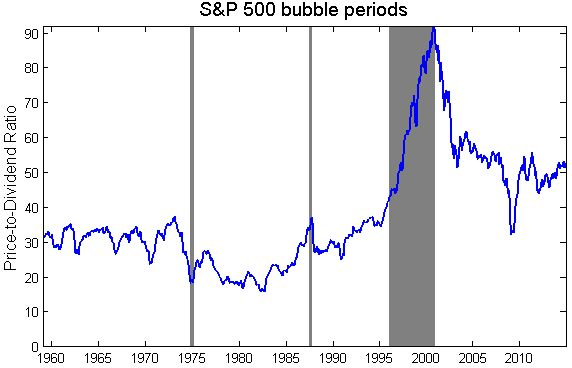
\includegraphics[width=\textwidth]{sp500bubble.jpg}
\end{figure}
\end{frame}

\begin{frame}
\frametitle{Stock and housing bubbles}
\begin{figure}[htb]
  \centering
    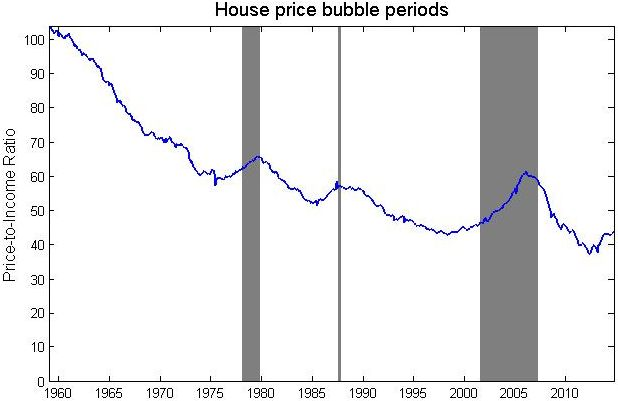
\includegraphics[width=\textwidth]{housebubble.jpg}
\end{figure}
\end{frame}

\begin{frame}
\frametitle{Forecast breakdowns of 12-month forecasts for output}
\begin{figure}[htb]
  \centering
    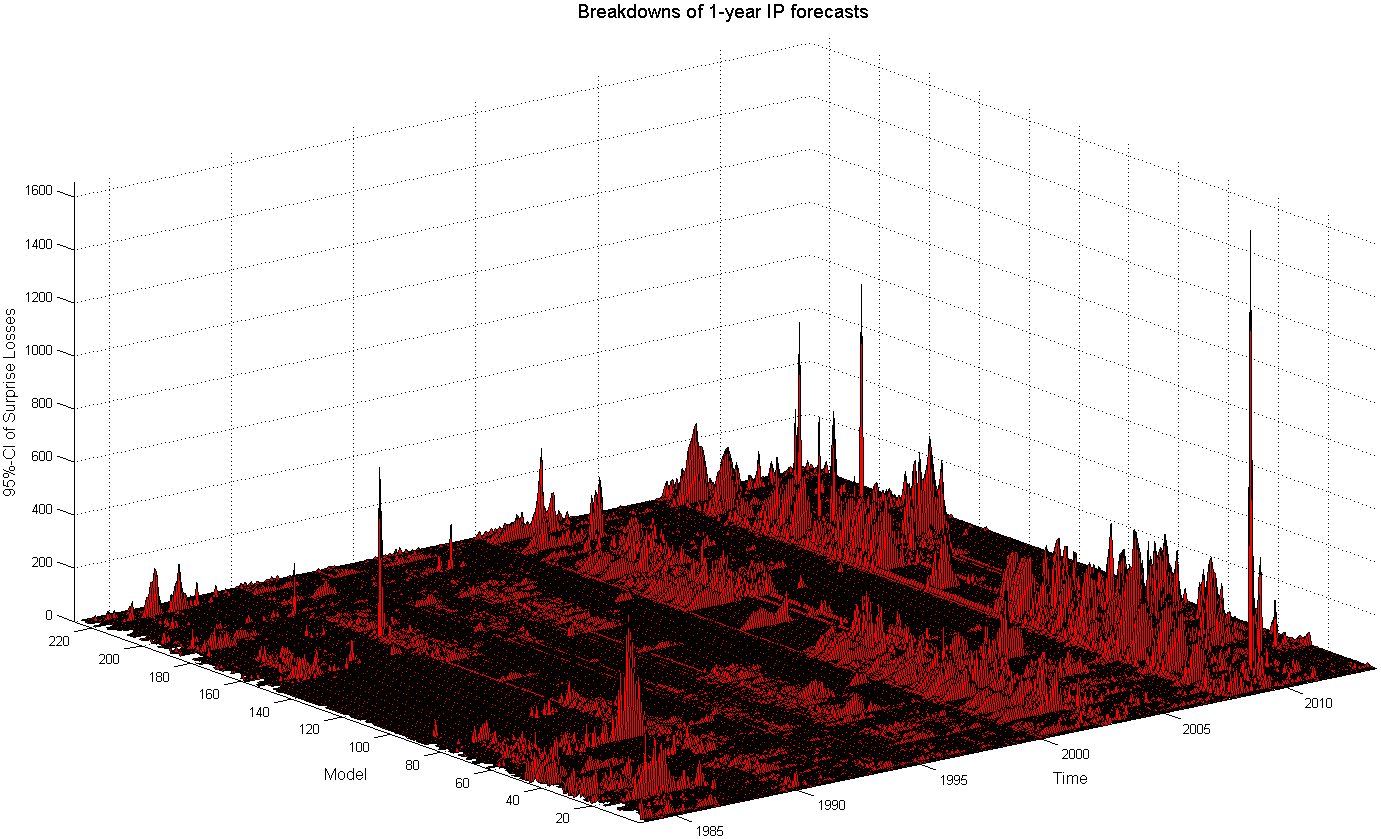
\includegraphics[width=\textwidth]{breakdowns.png}
\end{figure}
\end{frame}
		
%--------------------- Last Page ----------------------
\appendix
\newcounter{finalframe}
\setcounter{finalframe}{\value{framenumber}}
	
%-------- Literature ---------------------------------
\newcommand{\LastPageText}{Thank you.}
\begin{frame}[plain]
	\lastpage
\end{frame}

\begin{frame}[allowframebreaks]
\begin{small}
\bibliography{Bubbles_Breaks}
\end{small}
\end{frame}
%--------------------- Appendix ----------------------
%	\begin{frame}
%	\frametitle{References}
%		\bibliography{paper1}
%	\end{frame}

	
\end{document}